\section{Soddisfacimento degli obiettivi}
Al termine delle 320 ore di \textit{stage} presso \azienda{}, ho potuto effettuare una valutazione complessiva del lavoro svolto, 
focalizzandomi sul grado di raggiungimento degli obiettivi prefissati all'inizio dell'esperienza.

\begin{figure}[!h] 
  \centering 
  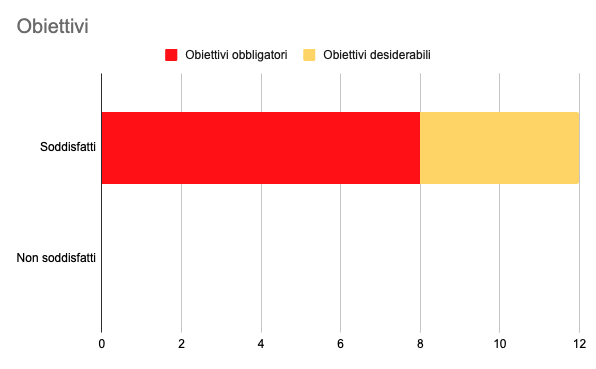
\includegraphics[width=.8\columnwidth]{obiettivi-soddisfatti} 
  \caption{Stato di completamento degli obiettivi.}
  \label{fig:obiettivi-soddisfatti}
\end{figure}

Come mostra la figura \ref{fig:obiettivi-soddisfatti}, sono riuscito a realizzare tutte le funzionalità obbligatorie che il piano di lavoro prevedeva (figura \ref{tab:obiettivi-obbligatori}),
in particolare ho realizzato:
\begin{itemize}
 \item Un \textit{plugin} per Gradle che analizza le dipendenze di un progetto;
 \item Un \textit{database} a grafo per memorizzare le dipendenze;
 \item Un \textit{backend} per esporre le funzionalità del \textit{plugin} tramite API \textit{REST} e per effettuare le interrogazioni al \textit{database};
 \item Un'interfaccia grafica per visualizzare le dipendenze e le relative versioni;
\end{itemize}

Ho realizzato anche tutte le funzionalità desiderabili (\ref{tab:obiettivi-desiderabili}), in particolare:
\begin{itemize}
\item Possibilita di visualizzare le dipendenze di un progetto in un formato grafico e non solo tabellare;
\item Integrazione con il \textit{repository} remoti per controllare la presenza di nuove versioni delle dipendenze;
\item Integrazione con il \textit{repository} remoti per controllare la presenza di vulnerabilità nelle dipendenze utilizzate;
\item Login tramite \textit{LDAP} per accedere all'interfaccia grafica;
\end{itemize}

In fine, ho realizzato anche alcune funzionalità aggiuntive, non previste nel piano di lavoro:
\begin{itemize}
  \item Possibilità di esplorare l'albero delle dipendenze in modo interattivo e \textit{lazy};
  \item Possibilità di effettuare ricerca di dipendenze tramite \textit{autocomplete}, mostrando la lista delle dipendenze che corrispondono alla ricerca raggruppate ;
  \item Possibilità di effettuare ricerche di dipendenze tramite \textit{query} \textbf{Cypher}, inserendo la \textit{query} nel campo di ricerca e visualizzando i risultati in un formato \textit{json};
\end{itemize}

La pianificazione iniziale delle ore per lo \textit{stage} prevedeva una distribuzione equilibrata tra le diverse fasi del progetto. 
Tuttavia, nel corso dello svolgimento, 
si sono verificate alcune variazioni significative. In particolare, il piano originale allocava circa tre settimane per lo sviluppo 
del \textit{frontend}, basandosi su stime \textit{standard} per questo tipo di lavoro.

Grazie alla mia consolidata esperienza con Angular, sono riuscito a ottimizzare notevolmente i tempi di sviluppo. 
Questa efficienza mi ha permesso di ridurre la durata prevista per questa fase, completando il lavoro in un arco temporale 
inferiore rispetto a quanto pianificato. La conseguenza diretta di questa accelerazione è stata la disponibilità di più 
tempo da dedicare ad altre attività fondamentali.

Ho sfruttato questa opportunità per approfondire la mia conoscenza delle tecnologie emergenti e partecipare a corsi di 
formazione aziendali. Questi corsi, offerti da \azienda{}, hanno arricchito il mio bagaglio di competenze.
